\documentclass[12pt]{beamer}
\usepackage{bookmark}
\usepackage[T1]{fontenc}

\usepackage{booktabs}
\usepackage{listings}
\lstset{basicstyle=\tiny}

\usepackage{tikz}
\usetikzlibrary{calc}
% tikzmark command, for shading over items
\newcommand{\tikzmark}[1]{\tikz[overlay,remember picture] \node (#1) {};}
\usepackage{mathtools}
\DeclareMathOperator*{\argmin}{arg\,min}
\DeclareMathOperator*{\argmax}{arg\,max}
\DeclareMathOperator*{\Var}{Var}
\DeclareMathOperator*{\diag}{diag}
\newcommand{\simiid}{\overset{\text{iid}}{\sim}}

\usepackage[bold]{hhtensor}
\newcommand{\vx}{\vec{x}}
\newcommand{\vy}{\vec{y}}
\newcommand{\cN}{\mathcal{N}}

\usepackage{pdfpages}
\usepackage{caption}

\usetheme[
    progressbar=foot,
    % sectionpage=none,
]{metropolis}
\setbeamercolor{background canvas}{bg=white}
\setbeamertemplate{note page}[plain]
% \setbeameroption{show notes on second screen=right}
%\setbeameroption{show only notes}

\usepackage{appendixnumberbeamer}

\title{Accelerating Metropolis-Hastings with Lightweight Inference Compilation}
\date{\today}
\author{Feynman Liang, Nim Arora, Nazanin Tehrani, Yucen Li, Michael Tingley, Erik Meijer}
\institute{Facebook Probability, Facebook AI Infrastructure, UC Berkeley}

\begin{document}

\maketitle

\begin{frame}{Table of contents}
  \setbeamertemplate{section in toc}[sections numbered]
  \tableofcontents%[hideallsubsections]
\end{frame}

\section{Background}

\subsection{Probabilistic Programming}

\begin{frame}[c]{Two competing philosophies}
    \cite{van2018introduction}
    To build machines that can reason,
    random variables and probabilstic calculations are:
    \\~\
    \\~\
    \pause
    \begin{columns}
    \begin{column}<+->{0.5\textwidth}
        \textbf{Probabilistic ML}

        An engineering requirement

        \cite{tenenbaum2011grow,ghahramani2015probabilistic}
    \end{column}
    \begin{column}<+->{0.5\textwidth}
        \textbf{Deep Learning}

        Irrelevant 

        \cite{lecun2015deep,goodfellow2016deep}
    \end{column}
    \end{columns}

    \note[item]{Automatic differentiation tools for the latter accelerated rapid exploration
    by offloading tedious gradient calculations to programming language tools}
    \note[item]{Necessity of programming tools for probabilistic ML motivates PPLs}
\end{frame}

\begin{frame}[fragile]{Probabilistic programming languages (PPLs)}
    \begin{quote}
        Just as programming beyond the simplest algorithms requires tools for abstraction and composition, complex probabilistic modeling requires new progress in model representation—probabilistic programming languages.
    \end{quote}
    \cite{goodman2013principles}
    \note[item]{Fundamentally about developing languages that allow
    \begin{enumerate}
        \item Specification of inference problems
        \item Evaluators to ``solve'' these problems
    \end{enumerate}
    }
\end{frame}

\begin{frame}[fragile]{Abstractions over deterministic computations}
    \begin{columns}
    \begin{column}[T]{0.5\textwidth}
        \textbf{Low Level Assembly}
        \begin{lstlisting}[language={[x86masm]Assembler}] 
mov  dx, msg
; ah=9 - "print string" sub-function
mov  ah, 9
int  0x21

"terminate program" sub-function
mov  ah, 0x4c
int  0x21

msg  db 'Hello, World!', 0x0d, 0x0a, '$'
        \end{lstlisting}
    \end{column}
    \pause
    \begin{column}[T]{0.5\textwidth}
        \textbf{High Level Python}
        \begin{lstlisting}[language=python]
print("Hello, World!")
        \end{lstlisting}
    \end{column}
    \end{columns}
    % \note[itemize]{
    %     \item Familiar: Abstraction / composition over assembly code, deterministic computations
    %     \item Easier to understand, debug, maintain; compiler can optimize as long as results consistent
    %     \item Same benefits for PPLs, but now for stochastic computations (reasoning under uncertainty)
    % }
\end{frame}

\begin{frame}[fragile]{Abstractions over probabilistic computations}

\begin{columns}
    \begin{column}<+->{0.4\textwidth}
        \centering
        \vspace{0.5cm}
        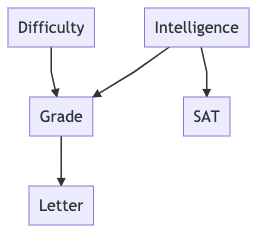
\includegraphics[width=\linewidth]{figures/student-network.png}
        \captionof{figure}{\cite{koller2009probabilistic}}
    \end{column}
    \begin{column}<+->{0.5\textwidth}
        \begin{verbatim}
        d ~ Bernoulli
        i ~ Normal
        g ~ g(d, i)
        s ~ s(i)
        l ~ Multinomial(g)
        \end{verbatim}
    \end{column}
\end{columns}

\note[item]{Probabilistic model for student recommendation letters and SAT scores}
\note[item]{Priors and conditionals}
\note[item]{Observations (Letter, SAT), Queries (Intelligence)}

\only<+>{\textbf{Generative model}: $P(D, I, G, S, L) = P(D) P(I) P(G \mid D, I) P(S \mid I) P(G \mid L)$ }
\only<.->{
    \begin{description}
        \item[Question]<+->: Given a student's recommendation \emph{letter} and \emph{SAT} score,
            what should I expect their \emph{intelligence} to be?
        \item[PPL Query]<+->: \texttt{infer(i, \{l=Good, s=800\})}
    \end{description}
}
\end{frame}

\subsection{Bayesian Inference}

\begin{frame}{Bayesian Inference Basics}
    \only<+-.(2)>{
    \begin{description}
        \item[Latent Variables] $X$
        \item[Observed Variables] $Y$
        \item[Prior] $P(X)$
        \item[Likelihood] $P(Y \mid X)$
    \end{description}
    }
    \only<+->{\alert{\textbf{Goal}: Approximate the posterior $P(X \mid Y)$}}
    \only<+>{
        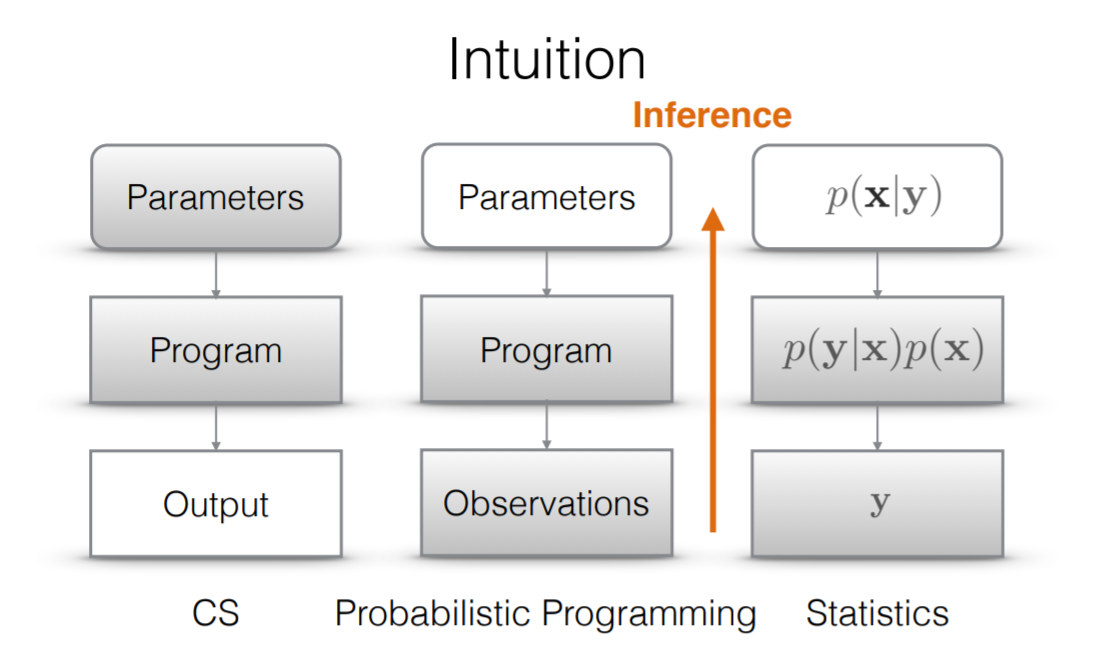
\includegraphics[width=0.9\textwidth]{figures/intuitive.png}
        \captionof{figure}{\cite{van2018introduction}}
    }
    \only<+>{
        \begin{tabular}{cc}
            \toprule
            $X$ & $Y$ \\
            \midrule
            intelligence & letter and grade \\
            scene description & image \\
            simulation & simulator output \\
            program source code & program return value \\
            policy prior and world simulator & rewards \\
            cognitive decision making process & observed behavior \\
            \bottomrule
        \end{tabular}
        \captionof{table}{\cite{van2018introduction}}
    }
\end{frame}

\begin{frame}{Why only approximate?}
    \[
        P(X \mid Y) 
        = \frac{P(Y \mid X) P(X)}{P(Y)}
        = \frac{P(Y \mid X) P(X)}{\underbrace{\int_X P(Y \mid X) P(X) dX}_{\eqqcolon Z(Y)}}
    \]
    \pause
    Denominator $Z(Y)$ (i.e. partition function, marginal likelihood $P(Y)$) high-dimensional integral, 
    known only for a small family of \emph{conjugate} prior/likelihood pairs
\end{frame}

\begin{frame}{How to approximate?}
    \begin{columns}
        \begin{column}[T]{0.5\textwidth}
            \only<+->{\textbf{Variational Inference}}

            \only<+->{
            Let $q_\phi$ be a tractable parametric family
            (e.g. Gaussian mean-field $q_\phi(X) = \prod_{i=1}^d N(X_i \mid \phi_{1,i},\phi_{2,i})$)
            }

            \only<+->{
            \begin{align*}
            &\argmin_\phi KL(q_\phi(X) \mid P(X \mid Y)) \\
            &= \argmax_\phi E_{q_\phi}\left[\frac{\log q_\phi(X)}{\log P(X \mid Y)}\right] \\
            &= \argmax_\phi E_{q_\phi}\left[\frac{\log q_\phi(X)}{\log P(Y \mid X) P(X)}\right]
            \end{align*}
            }
        \end{column}

        \begin{column}[T]{0.5\textwidth}
            \tikzmark{montecarlo}{
                \only<1->{\textbf{Monte Carlo}}

                \only<+->{
                Sample $X_i \overset{\text{iid}}{\sim} P(X \mid Y)$. Then
                }
                \only<+->{
                \begin{align*}
                    & \mathbb{E}[g(X) | Y] \\
                    & = \int g(X) \cdot P(X \mid Y) dX \\
                    & \approx \frac{1}{N} \sum_{n=1}^N g(X_i)
                \end{align*}
                }
            }
        \end{column}
    \end{columns}
    \pause\tikz[overlay,remember picture]{\draw[draw=red,thick,double,fill opacity=0.2] ($(montecarlo)+(-0.5,0.4)$) rectangle ($(montecarlo)+(5.5,-5.2)$);}

    \note[item]{Integrals are just really tiny sums, CLT $1/\sqrt{N}$ rate}
    \note[item]{Can answer this question by drawing samples from the posterior, inference is solved by sampling the posterior}
\end{frame}

\section{Inference compilation in declarative PPLs}

\subsection{SIS in imperative PPLs}

\begin{frame}[fragile]{Imperative vs Declarative PPLs}
    \textbf{Imperative}: Evaluation-based, samples (linear) execution traces
        (Pyro, Church, WebPPL)
    \pause
    \begin{lstlisting}[language=lisp]
(begin
    (define geometric
        (lambda (p)
        (if (flip p)
        1
        (+ 1 (geometric p)))))
    (geometric .7))
        \end{lstlisting}

        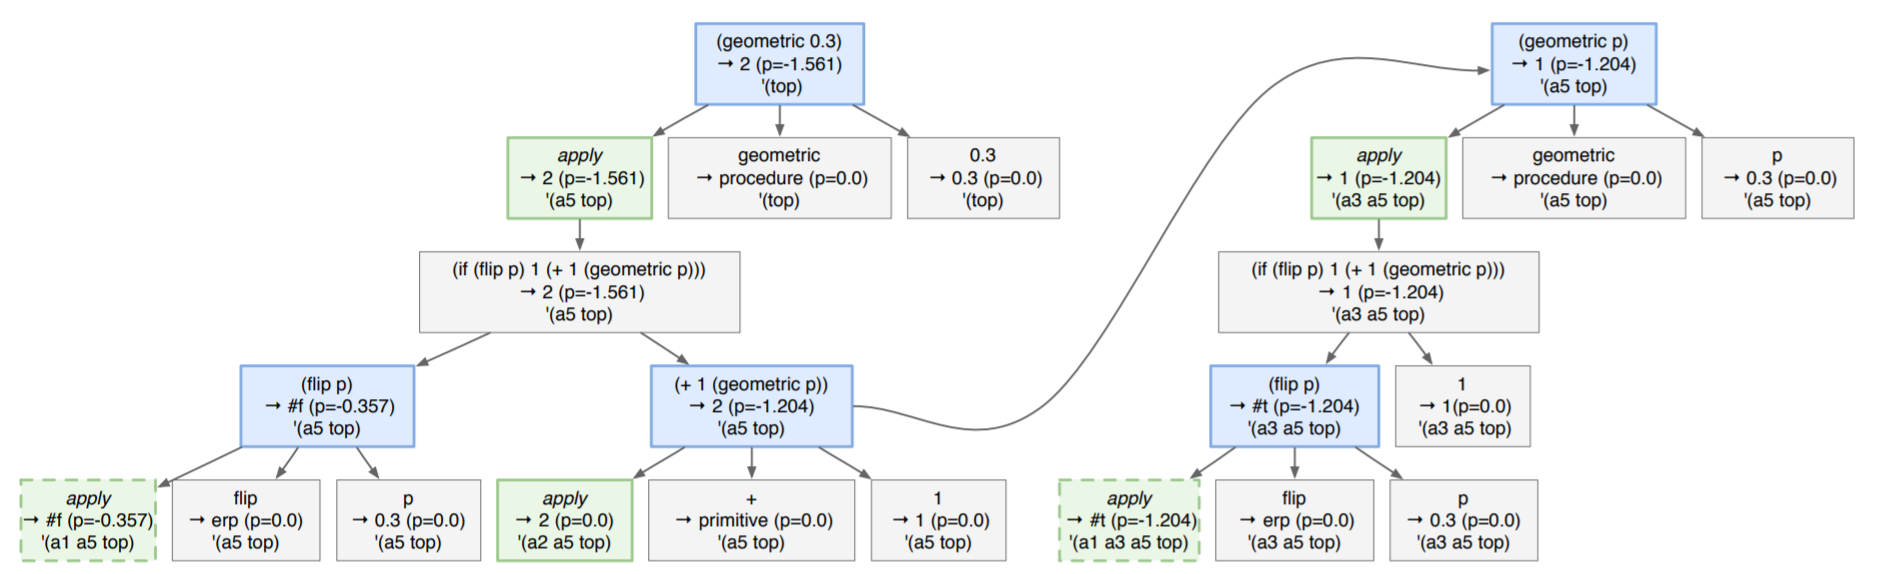
\includegraphics[width=1.0\textwidth]{figures/execution-trace.png}
        \captionof{figure}{\cite{wingate2011lightweight}}
\end{frame}

\begin{frame}{Sequential importance sampling (SIS)}
    If we can sample $X_i \sim q$ from proposal distribution $q$,
    \pause
    \begin{align*}
        \mathbb{E}_{P(X \mid Y)}[g(X)]
        &= \mathbb{E}_{P(X \mid Y)}\left[\frac{q(X)}{q(X)} g(X)\right]
        = \frac{\mathbb{E}_{q}\left[\frac{P(X,Y)}{q(X)} g(X)\right]}{P(Y)} \\
        &\approx \frac{1}{N} \sum_{i}^N \frac{\frac{P(X_i,Y)}{q(X_i)}}{P(Y)} g(X_i)
        \approx \sum_{i}^N \frac{\frac{P(X_i,Y)}{q(X_i)}}{\sum_i^N \frac{P(X_i, Y)}{q(X_i)}} g(X_i)
    \end{align*}
    \pause
    Convergence rate $\Var_q\left[\frac{P(X, Y)}{q(X)} g(X)\right]^{-1/2}$ \cite{yuan2007theoretical}
\end{frame}

\begin{frame}{SIS of execution traces}
    \begin{enumerate}
        \item Execute the probabilistic program forwards
        \item At each stochastic variable (i.e. \texttt{sample} statement),
            sample from proposer $q(\cdot)$ and assign value
        \item At each observed random variable (i.e. \texttt{observe} statement),
            multiply likelihood into trace's importance weight
    \end{enumerate}
    \pause

    \textbf{Problem}: Myopic choices from sampling $q$ early in the trace
    may result in low importance weights later. Would like $q$ to account
    for observations $Y$.
\end{frame}

\begin{frame}[fragile]{Constructing a proposal distribution}
    How to choose $q$? 
    
    \pause
    \textbf{Likelihood-Weighting \cite{norvig2002modern}}: $q(X) = P(X)$

    \pause
    \textbf{Direct sampling}: $q(X) = P(X \mid Y)$, optimal
    
    \pause
    \textbf{Key Idea}: Exploit access to $P(X,Y)$ to
    build a proposer $q$ ``close'' to $P(X \mid Y)$?
\end{frame}

\begin{frame}{Trace-based inference compilation (IC)}
    \begin{itemize}
        \item Construct DNN with parameters $\phi$
        mapping observations $Y$ (amortized inference, \cite{goodman2013principles})
        and execution prefix to proposal distribution $q_\phi(\cdot \mid Y)$ 
        \item Train $q_\phi$ against forward samples from the probabilistic program
            $p(x,y)$ (inference compilation)
    \end{itemize}

    \centering
    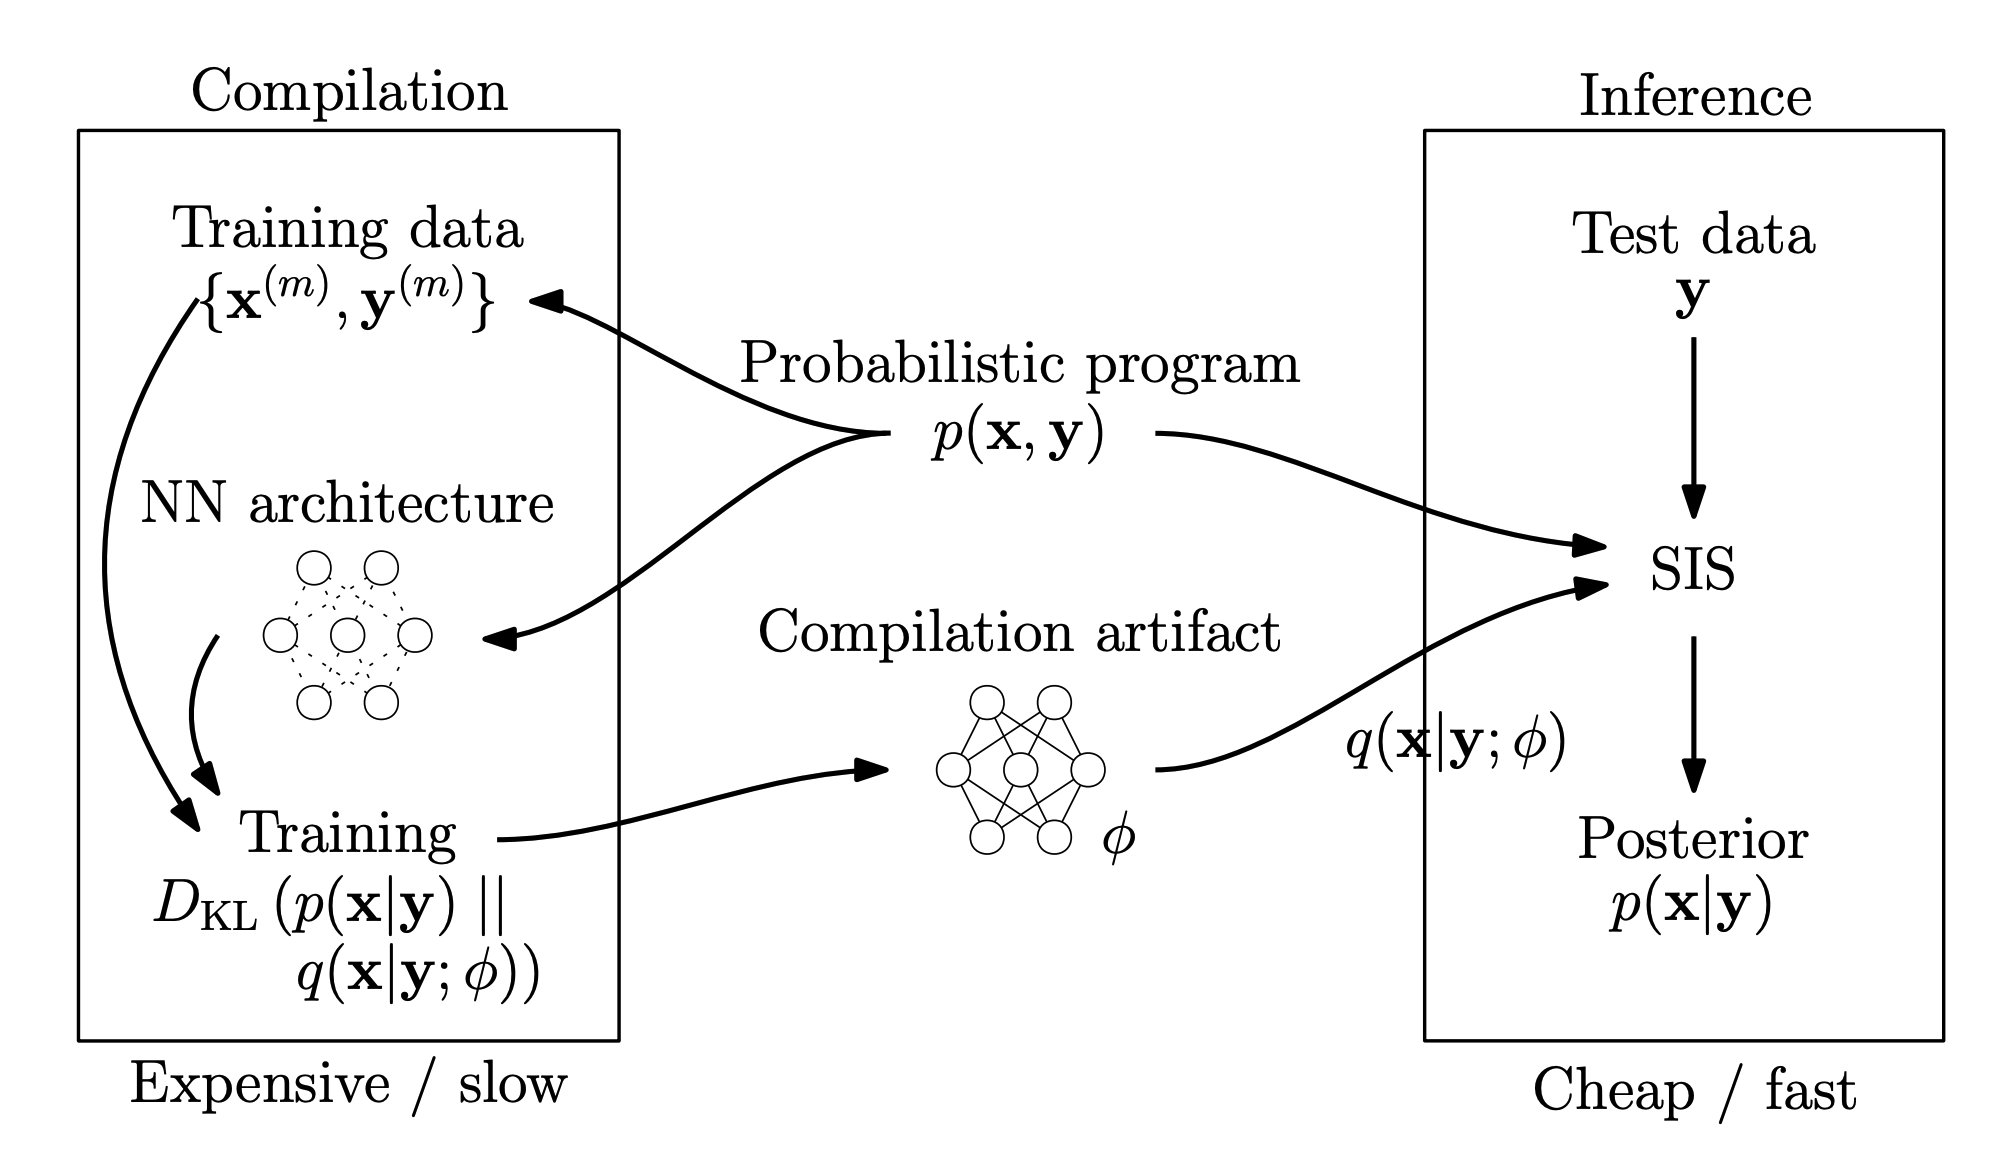
\includegraphics[width=0.6\linewidth]{figures/ic.png}
    \captionof{figure}{\cite{le2017inference}}
\end{frame}

\begin{frame}{Intuition for inference compilation}
    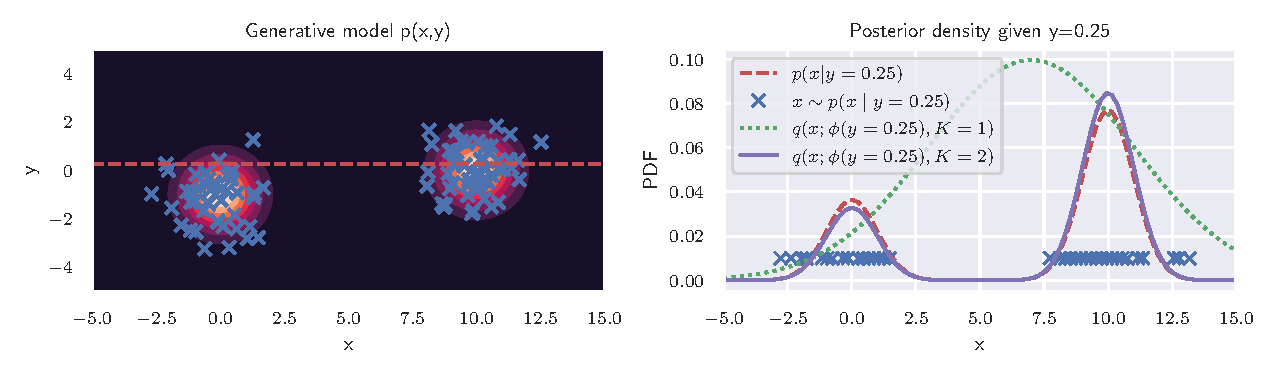
\includegraphics[width=\textwidth]{figures/intuition.pdf}
\end{frame}

\begin{frame}{Trace-based inference compilation (IC)}
    \centering
    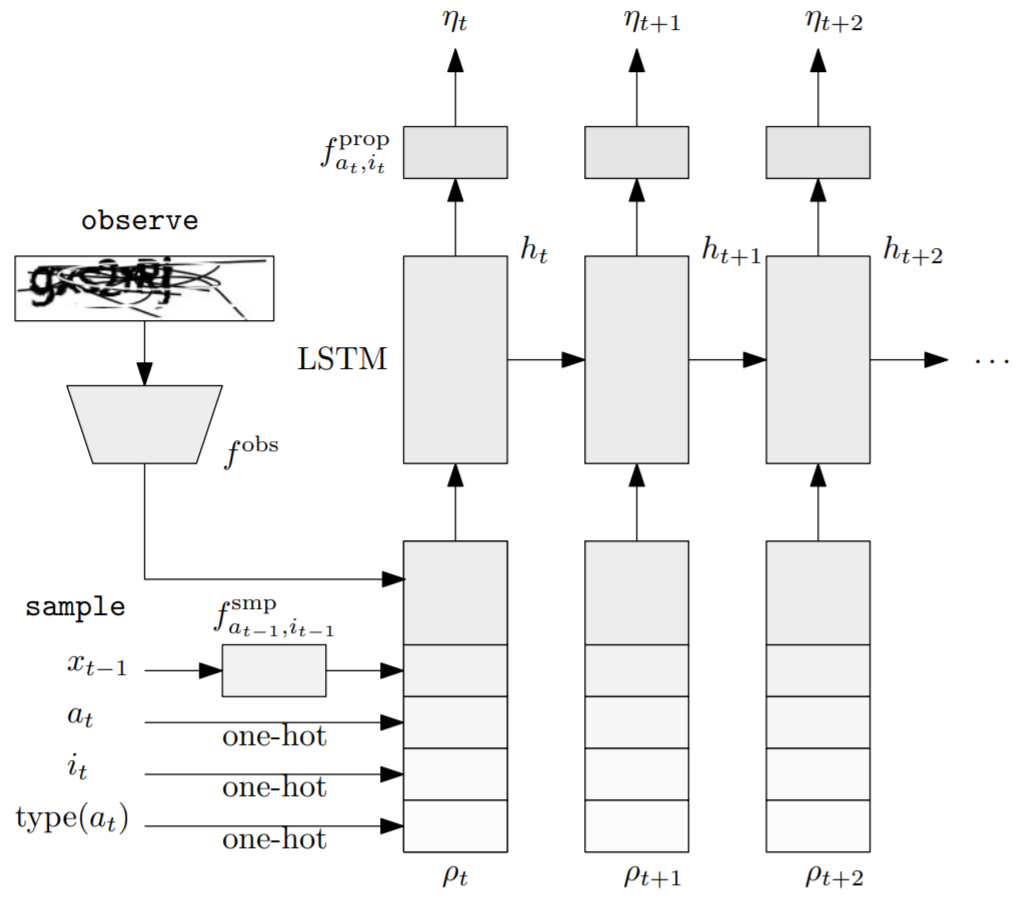
\includegraphics[width=0.7\linewidth]{figures/ic-lstm.png}
    \captionof{figure}{\cite{le2017inference}}
\end{frame}

\begin{frame}[fragile]{Sensitivity to nuisance random variables}
    \begin{lstlisting}[language=Python]
def magnitude(obs, M):
    x = sample(Normal (0, 10))
    [sample(Normal (0 ,10)) for _ in range(M)] # extend trace with nuisance
    y = sample(Normal (0 ,10))
    observe(obs**2, Likelihood=Normal(x**2 + y**2, 0.1)0
    return x, y
    \end{lstlisting}

    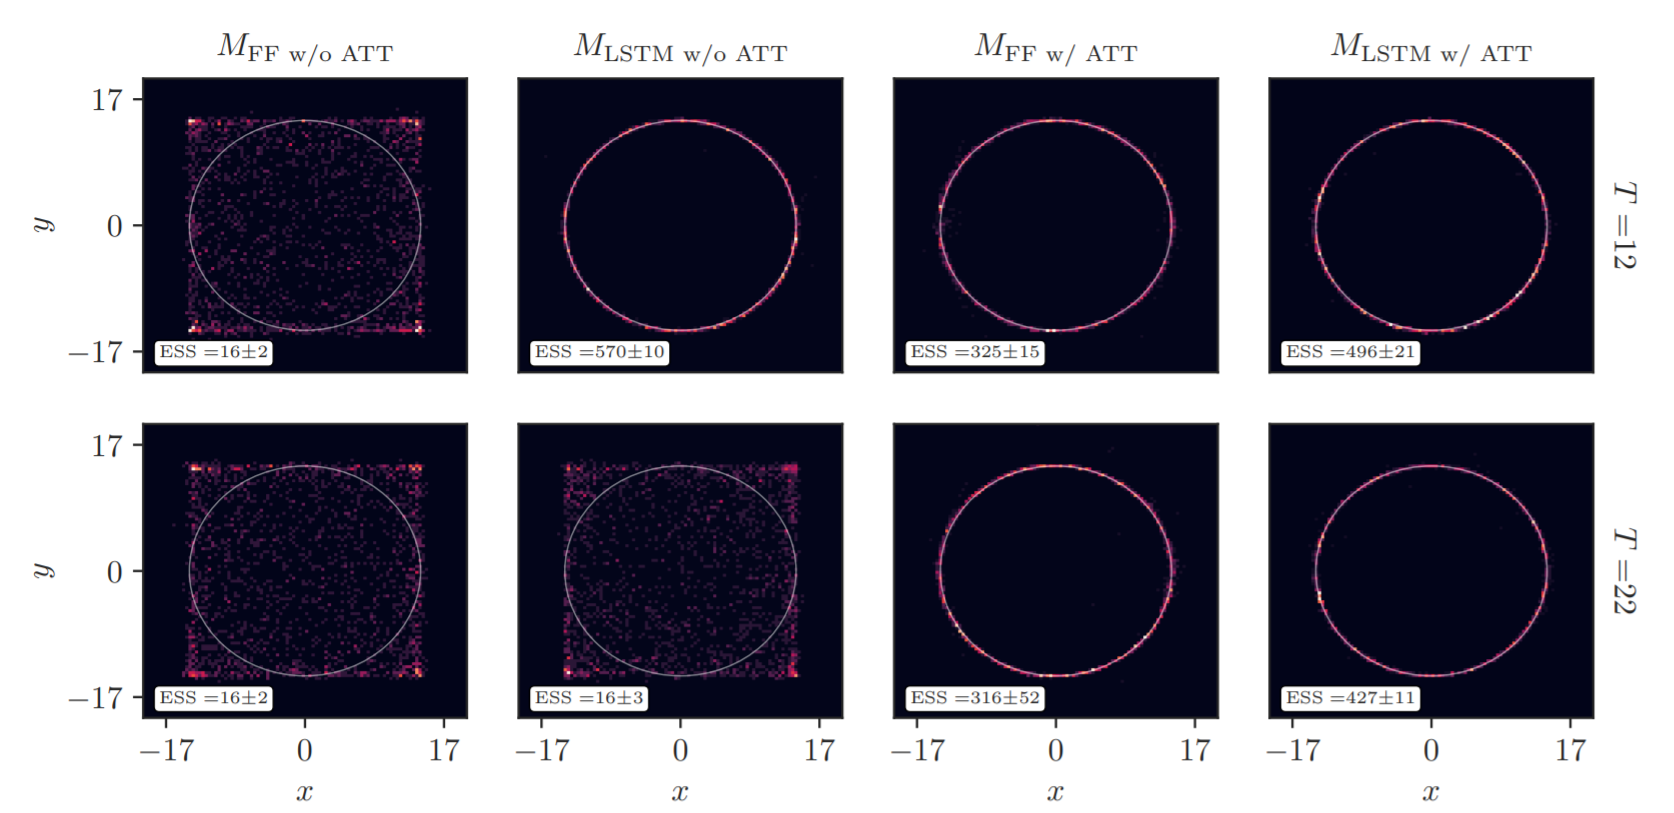
\includegraphics[width=0.9\textwidth]{figures/attention.png}
    \captionof{figure}{\cite{harvey2019attention}}
\end{frame}

\subsection{Lightweight Inference Compilation for MCMC}

\begin{frame}{Imperative vs Declarative PPLs}
        \textbf{Declarative}: Graph-based, samples instantiated graphical models (i.e. worlds)
            (BUGS, BLOG, Stan, beanmachine)

        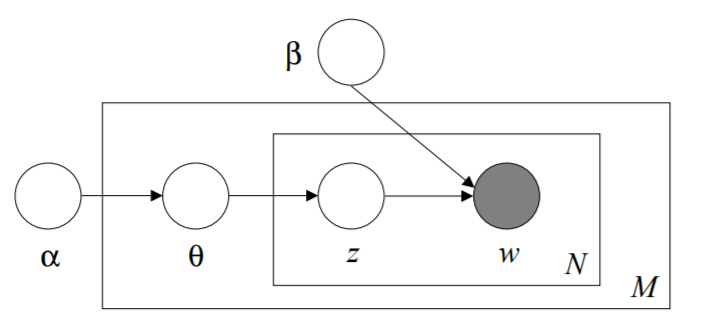
\includegraphics[width=0.8\textwidth]{figures/LDA.png}
        \captionof{figure}{\cite{blei2003latent}}

        \textbf{Key Idea}: Markov blanket $\text{MB}(X_i)$ available in
        declarative PPL
\end{frame}

\begin{frame}[fragile]{MCMC sampling of graphical models}
    Metropolis-within-Gibbs / Lightweight MH (\cite{wingate2011lightweight}):
    \begin{itemize}
        \item Fix observed nodes $Y$ to their values.
        \item Repeat:
        \begin{itemize}
            \item Pick single random unobserved node $X_i$
            \item Sample proposal $q(X_i)$ to propose new value
            \item Accept with probability $\alpha$ and revert otherwise
        \end{itemize}
    \end{itemize}

    \pause
    
    \begin{theorem}[\cite{hastings1970monte}]
        With appropriately chosen $\alpha$, the above algorithm yields
        a Markov Chain with the posterior as the invariant distribution.
    \end{theorem}

\end{frame}

\begin{frame}[fragile]{MH proposal distributions}
    Different $q(\cdot)$ $\implies$ different MCMC algorithms
    
    \begin{itemize}
        \item<+-> Random walk MH: $q(\cdot)$ isotropic Gaussian
        \item<+-> Newtonian Monte Carlo \cite{arora2020newtonian}: $q(\cdot) =$ Gaussian
            with empirical Fisher information
        \item<+-> Hamiltonian Monte Carlo: $q(\cdot)$ integrates iso-Hamiltonian system
        \item<+-> Lightweight Inference Compilation: $q(\cdot \mid \text{MB}(X_i))$ a neural network
            function of the current Markov Blanket
    \end{itemize}

    \onslide<+->
    \begin{theorem}[\cite{pearl1987evidential}]
        Gibbs distributions $P(X_i \mid X_i^c) = P(X_i \mid \text{MB}(X_i))$
        are optimal proposers $q(\cdot)$
    \end{theorem}

    \onslide<+->
    $\therefore$ $\text{MB}(X_i)$ is the minimal sufficient inputs for generating proposal distribution
\end{frame}

\begin{frame}[fragile]{LIC artifacts for example student network}
    \begin{minipage}{0.4\linewidth}
        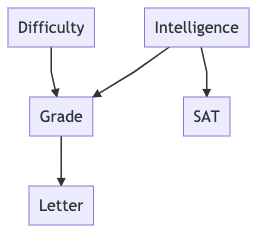
\includegraphics[width=\linewidth]{figures/student-network.png}
    \end{minipage}
    \begin{minipage}{0.5\linewidth}
        \begin{align*}
            & q(d | g, i) \\
            & q(i | g, d, s) \\
            & q(g | i, d, l) \\
            & q(s | i) \\
            & q(l | g)
        \end{align*}
    \end{minipage}
    \note[item]{
    Each IC proposer only has access to Markov Blanket, respects causal structure
    }
    \note[item]{
    SIS IC suffers in presence of nuisance parameters, requires attention to perform well
    }
    \note[item]{
    Explain declarative vs imperative (parents are clearly demarcated)
    }
\end{frame}

\begin{frame}[fragile]{Example LIC proposer for grade}

    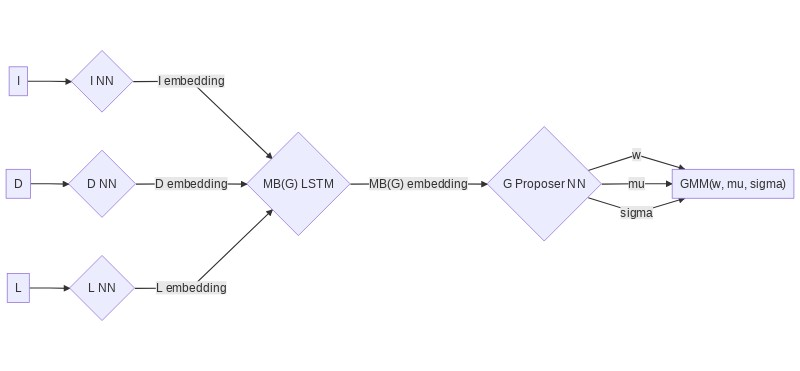
\includegraphics[width=\textwidth]{figures/ic-grade.png}
% graph LR
%   I[intelligence] --> Ie{intelligence FFW NN}
%   D[difficulty] --> De{difficulty FFW NN}
%   L[letter] --> Le{letter FFW NN}
% 	Ie -->|intelligence  embedding vector| MB{Markov blanket LSTM}
%   De -->|difficulty embedding vector| MB
%   Le -->|letter embedding vector| MB
%   MB -->|Markov blanket embedding| P{proposer FFW NN}
%   P -->|w| Q["Q(grade) = GMM(w, mu, sigma)"]
%   P -->|mu| Q
%   P -->|sigma| Q

\note[itemize]{
    \item Markov blanket can change size due to switching variables => LSTM
    \item Problem: density estimator currently Gaussian/Categorical
    \item Problem: observations shape fixed at compile
}
\end{frame}

\begin{frame}{Compare against SIS IC's (non-minimal) proposer}
\begin{columns}
    \begin{column}{0.4\linewidth}
        \centering
        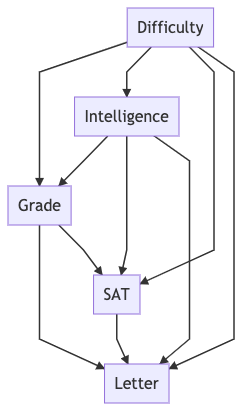
\includegraphics[width=\linewidth]{figures/student-network-smc-ic.png}
    % graph TD
    %   D[Difficulty] --> G[Grade]
    %   D --> I
    %   D --> S
    %   D --> L
    %   I[Intelligence] --> G
    %   I --> S[SAT]
    %   I --> L
    %   G --> L[Letter]
    %   G --> S
    %   S --> L
    \end{column}
    \begin{column}{0.5\linewidth}
        \begin{align*}
            & q(d | \text{observations}) \\
            & q(i|d, \text{observations}) \\
            & q(g | i, d, \text{observations}) \\
            & q(s | g, i, d, \text{observations}) \\
            & q(l | s, g, i, d, \text{observations})
        \end{align*}
    \end{column}
\end{columns}
\end{frame}


\section{Results}

\begin{frame}{Recovering conjugate expressions in normal-normal}
    \centering
    $x \sim N(0, 2)$, $y \mid x \sim N(x, 0.1)$

    \textbf{Know}: $y \mid x \sim N(0.999x, 0.0001)$

    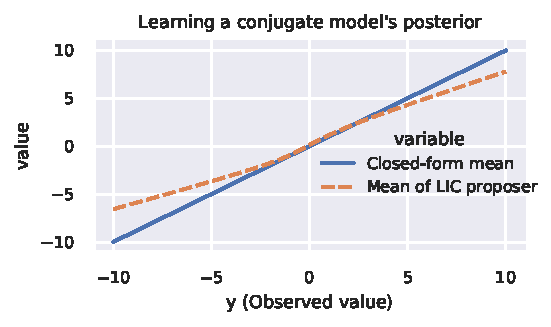
\includegraphics[width=0.8\textwidth]{figures/normal_normal_mean.pdf}
\end{frame}

\begin{frame}{GMM Mode Escape}
    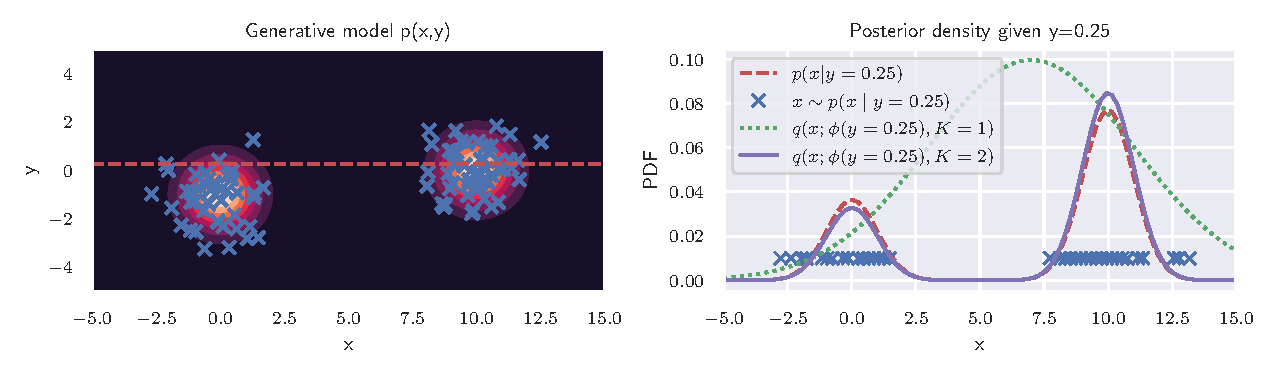
\includegraphics[width=\textwidth]{figures/intuition.pdf}
    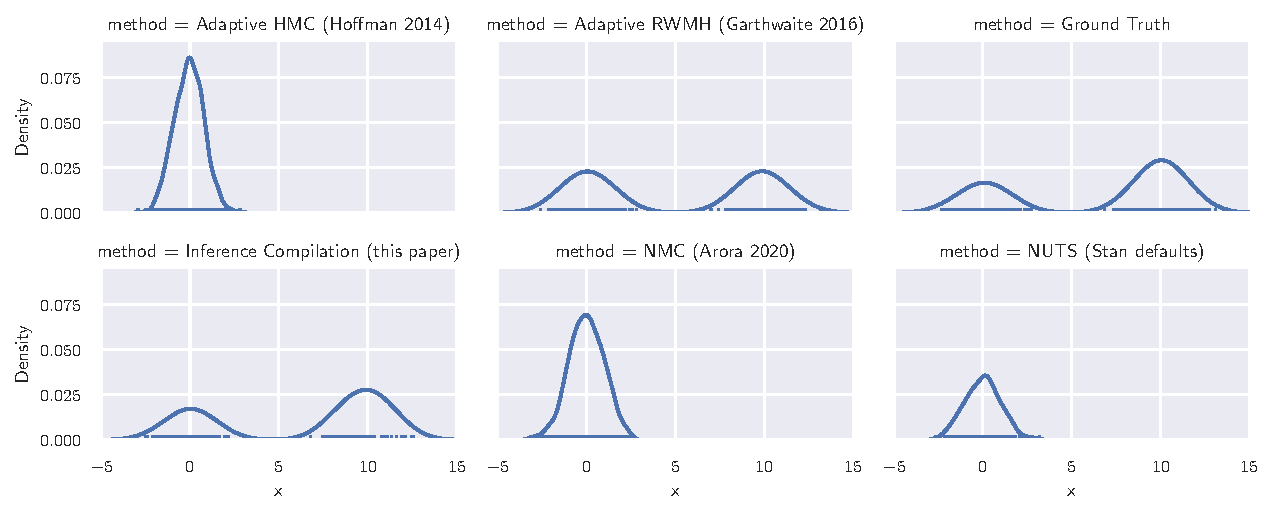
\includegraphics[width=\textwidth]{figures/mode_escape.pdf}
\end{frame}

\begin{frame}[fragile]{Robustness to nuisance random variables}
    \begin{columns}
        \begin{column}{0.5\textwidth}
\begin{lstlisting}[language=Python]
def magnitude(obs):
  x = sample(Normal(0, 10))
  for _ in range(100):
    nuisance = sample(Normal(0, 10))
  y = sample(Normal(0, 10))
  observe(
    obs**2,
    likelihood=Normal(x**2 + y**2, 0.1))
  return x
\end{lstlisting}
        \end{column}
        \begin{column}{0.5\textwidth}
\begin{lstlisting}[language=Python]
class NuisanceModel:
  @random_variable
  def x(self):
      return dist.Normal(0, 10)
  @random_variable
  def nuisance(self, i):
      return dist.Normal(0, 10)
  @random_variable
  def y(self):
      return dist.Normal(0, 10)
  @random_variable
  def noisy_sq_length(self):
      return dist.Normal(
          self.x()**2 + self.y()**2, 
          0.1)
\end{lstlisting}
        \end{column}
    \end{columns}
    \begin{tabular}{lccc}
        \toprule
                            & \# params & compile time & ESS   \\
        \midrule
        LIC (this paper)       & 3,358     & 44 sec.      & 49.75 \\
        \cite{le2017inference} & 21,952    & 472 sec.     & 10.99 \\
        \bottomrule
    \end{tabular}
\end{frame}

\begin{frame}{Bayesian Logistic Regression}
    $\vec{\beta} \sim \cN_{d+1}(\vec{0}_{d+1}, \diag(10, 2.5\vec{1}_{d}))$,
    $y_i \mid \vx_i \simiid \text{Bernoulli}(\sigma(\vec{\beta}^\top \vx_i))$
    where $\sigma(t) = (1 + e^{-t})^{-1}$

    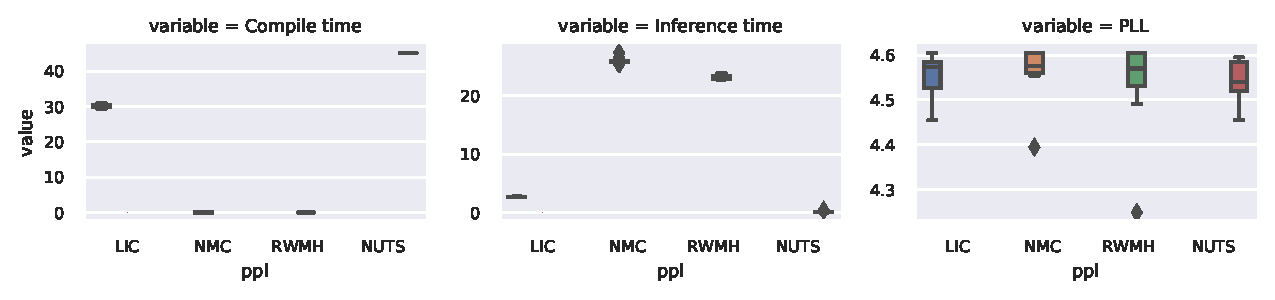
\includegraphics[width=\textwidth]{figures/blr_pll.pdf}
    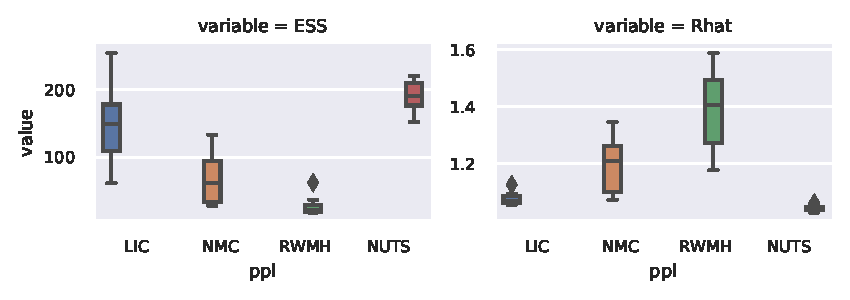
\includegraphics[width=0.66\textwidth]{figures/blr_ess_rhat.pdf}
\end{frame}

\begin{frame}{n-Schools}
    \only<1>{\begin{align*}
        \beta_0     & \sim \text{StudentT}(3, 0, 10)                                                                         \\
        \tau_{i}    & \sim \text{HalfCauchy}(\sigma_i) \qquad \text{for}~i \in [\text{district}, \text{state}, \text{type}]  \\
        \beta_{i,j} & \sim \cN(0, \tau_i)  \qquad \text{for}~i \in [\text{district}, \text{state}, \text{type}], j \in [n_i] \\
        y_k         & \sim \cN(\beta_0 + \sum_i \beta_{i,j_k}, \sigma_k)
    \end{align*}}
    \only<2>{
        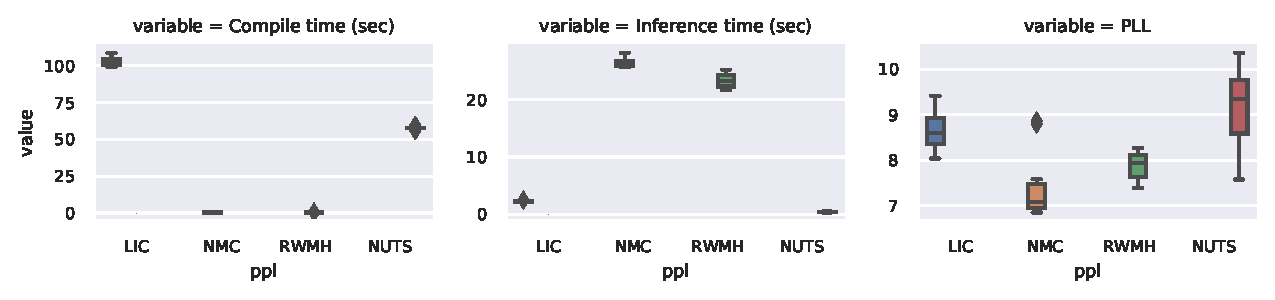
\includegraphics[width=\textwidth]{figures/nschools_pll.pdf}
        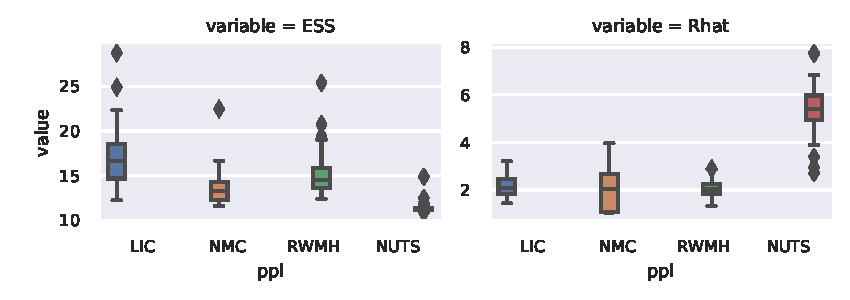
\includegraphics[width=0.66\textwidth]{figures/nschools_ess_rhat.pdf}
    }
\end{frame}

\section{Future directions}

\begin{frame}{Adaptive LIC}
    \textbf{Problem}: forward samples during compilation may not sufficiently represent observations ($\text{obs}$) encountered at inference

    RWMH adapts step size \cite{garthwaite2016adaptive}, HMC adapts
    mass matrix \cite{hoffman2014no}, can LIC adapt NN weights?

    \textbf{Solution}: perform MCMC with IC artifact to draw posterior samples $(\vec{x}^{(m)}, \vec{y}^{(m)}=\text{obs}) \sim P(\vec{x} \mid \vec{y}=\text{obs})$,
    hill-climb inclusive KL between \emph{conditional} (rather than joint) posterior
    \begin{align*}
        &\argmin_{\phi} D_{KL}(p(\vec{x} | \vec{y}=\text{obs}) || q(\vec{x} | \vec{y}=\text{obs}; \phi)) \\
        &\approx 
        \argmin_{\phi} \sum_{m=1}^N \log Q(\vec{x}^{(m)} \mid \vec{y} = \text{obs}, \phi)
    \end{align*}
\end{frame}

\begin{frame}{IAF density estimators}
    \textbf{Problem}: GMM in LIC may not be as expressive
    as more recently developed density estimators \cite{kingma2016improved}

    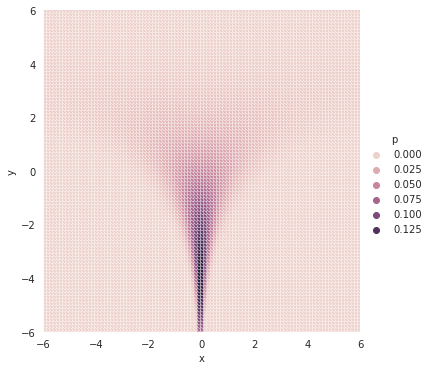
\includegraphics[width=0.3\textwidth]{figures/neal_funnel.png}
    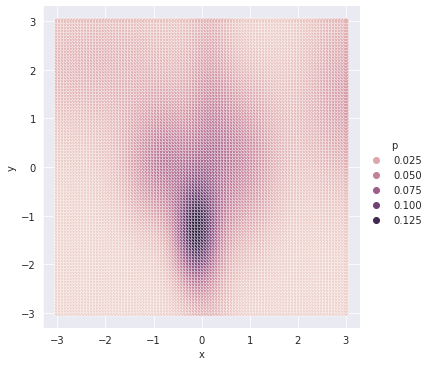
\includegraphics[width=0.3\textwidth]{figures/neal_funnel_gmm.png}
    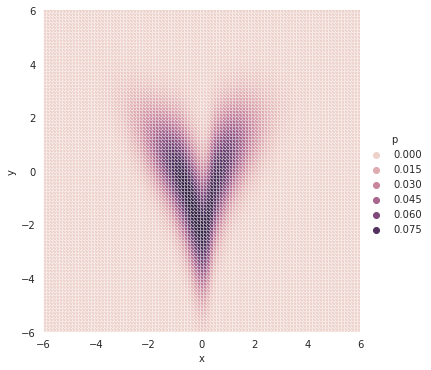
\includegraphics[width=0.3\textwidth]{figures/neal_funnel_iaf.png}
    \captionof{figure}{Neal's funnel (left) and a 7-component isotropic GMM
    (middle) and 7-layer IAF (right) density approximation}
\end{frame}

\begin{frame}{Heavy-tailed density estimators}
    \textbf{Problem}: GMMs and standard IAFs (Lipschitz functions of Gaussians) remain sub-Gaussian,
    $n$-schools is heavy tailed

    \textbf{Idea}: IAFs with heavy-tailed base distribution
    \begin{columns}
        \begin{column}{0.4\textwidth}
            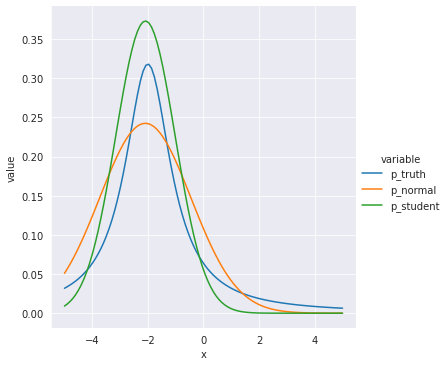
\includegraphics[width=\textwidth]{figures/heavy_tailed_iaf.png}
        \end{column}
        \begin{column}{0.3\textwidth}
            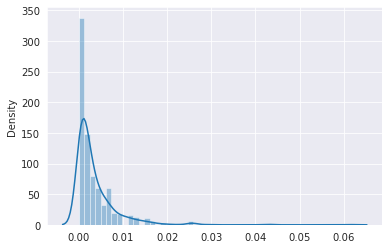
\includegraphics[width=0.9\textwidth]{figures/heavy_tailed_iaf_normal_ks.png}
            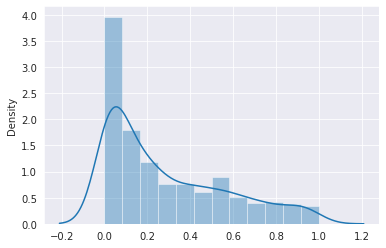
\includegraphics[width=0.9\textwidth]{figures/heavy_tailed_iaf_studentt_ks.png}
        \end{column}
    \end{columns}
    \captionof{figure}{IAF density estimation of a $\text{Cauchy}(-2, 1)$ (left) and their
    K-S statistics when using a Normal (right top) and StudentT (right bottom) base distribution}
\end{frame}


\begin{frame}[allowframebreaks]{References}
  \bibliography{refs}
  \bibliographystyle{apalike}
\end{frame}

\end{document}
